\documentclass[8pt]{article}
\title {Predicting the number of deaths related 
to COVID-19 in Italy and Germany}

\usepackage{graphicx}
\usepackage{verbatim}
\usepackage{amsthm}
\usepackage{amssymb}
\usepackage{amsmath}
\newtheorem{deff}{Definition}
\usepackage{graphicx}
\usepackage{subcaption}
\usepackage[font=small,labelfont=bf]{caption}


\newcommand{\norm}[1]{\left\lVert#1\right\rVert}
%\newtheorem{theorem}{Proposition}
\newtheorem{definition}{Definition}
\newtheorem{Proposition}{Proposition}

\begin{document}
\maketitle
\section{Introduction}
One direct way to measure an epidemics impact is to quantify the number 
of victims.
We aim at mathematically describing its evolution
in time $X(t) = X^P(t)$ by using a generalized logistic model, so that 
we infer the value of $P$ by observing the official datasets.


Instead of looking for precise values of $P$, we adopt a probabilistic
viewpoint when we embrace an \emph{uncertainty} around them, quantified
by using Bayesian techniques. The $pCN$ Markov Chain Monte Carlo is used
for this task, showing its effectiveness for this concrete finite
dimensional example. The results are sum up into a probability
measure for $P$: by choosing the parameters corresponding
to the "worst" and the "best" scenario, we draw curves in time, delimiting the
area in which we expect the future data to oscillate.


Concretely speaking, we analyze the situations in Germany and Italy.
Briefly speaking both the country had lockdown measures for the month
of April, expected to be still valid until the mid of May, when new
changes are planned.


Our question might be formulated as follows:
for how many days in April do we have to collect data,
before being able to predict the evolution until the mid of May? 
Our conjecture is that such a number is only
model dependent, therefore the same for all
the analyzed Countries. In case of success, this knowledge can be
exploited for the future possible scenario.



\section {Our generalized logistic model}
We choose to model the number of deaths in time by a 
specific generalized logistic function. 
All the maps in this family are
 $S$-shaped curves with an exponential starts
slowed down until reaching an almost constant horizontal phase. 


We do not provide any deep epidemiological explanation for such a choice,
except that we expect a similar qualitative behavior for the phenomenon
under analysis: the number of deaths is supposed to be higher at the beginning,
reaching then a saturation point as long as the health system becomes
capable of managing the emergency.
Successful applications in similar contexts can be found in REF.


Our general ODE logistic map is given by the following equation:

\begin{equation}
	X'(t) = \frac{q}{v} X(t) 
	\left ( 1 - \left( \frac{X(t)}{Q} \right)^{v}\right )
\end{equation}
with closed form solution:
\begin{equation}
	X(t) = \frac{Q} { (1 + A \exp[-q t])^{\frac{1}{v}}}
\end{equation}

for three real parameters, 
$P = \{ q, Q, v\}$ and initial time zero condition $X_0$,
(we write $X(t) = X^P(t) = X^P_{X_0}(t)$ to stress this dependence).
Here $A$ abbreviates 
$A = -1 + \left ( \frac{Q} { X_0} \right )^{v}$.


Due to the limit $\lim_{t \to \infty} X(t) = Q$, 
we interpret $Q$ as
the maximum value reached asymptotically, sometimes
referred as the \emph{carrying capacity} in the literature.
In our case, it is certainly positive $Q > 0$.


The parameter $v > 0$ is related to the symmetry of the curve.
Its limit for $v \to 0^+$ produces the \emph{Gompertz} model,
while the case $v = 1$ the \emph{simple} logistic map.
Both these simpler models are widely used in the literature, REF.


Finally, an asymptotically analysis as shown in REF 
describes $q > 0$ as the coefficient for the initial exponential 
growth.

\begin{comment}
\subsection {The simple logistic map}
In the simple logistic map the model $X^P(t)$ depends on two real positive
parameters, $P = \{ q, Q \}$, so that $n = 2$,
and is the solution of the 1-dimensional ODE:
\begin{equation}
	X'(t)  = q X(t) \left ( 1 - \frac{X(t)}{Q} \right )
\end{equation}
with closed-form formula:
\begin{equation}
X(t) = \frac{X_0 \exp[q t]}
	{1-\frac{X_0}{Q} (1-\exp[q t)])}
\end{equation}


Where again $X_0$ is the starting ODE condition at time $0$.
Of course, we have $\lim_{t \to \infty} X(t) = Q$,
and since this simple logistic map is equivalent to the simplest SIS
model (as explained before), the parameter $q$ can be actually
rigorously related to the average number of daily people's social interaction.


\subsection{The Gompertz law}
The Gompertz law is governed by two real positive parameters,
$q$ and $Q$, therefore we write again $P = \{q, Q\}$ and $n = 2$.
Once the starting condition $X_0$ at time zero
is specified, $X(t) = X^P(t) = X_{X_0}^P(t)$ is the solution to:

\begin{equation}
 X'(t) = q X(t) \log \left [\frac{Q} {X(t)} \right ]
\end{equation}
expressed by the closed-form formula:
\begin{equation}
X(t) = Q \exp	\left [
	\log \left [ \frac{X_0}{Q} \right ]
	\exp \left [ -q t \right ]
		\right ]
\end{equation} 


As seen for the previous cases, $Q$ corresponds to the limit
$\lim_{t \to \infty} X(t)$.
\end{comment}

\section{The bayesian approach}
Let $X^P_{X_0}(t)$ be always the generalized logistic model depending on
parameters $P$ and with $X_0$ time zero condition.
When using the models in practice, we can only observe a
limited amount of points coming from its ODE trajectory, 
which are furthermore perturbed by a (random) noise.
Let's fix $T+1$ times $\{t_i\}_{i = 0,\dots, T}$.
\begin{definition}
	The \emph{observed vector} $\textbf{y} \in \mathbb{R}^{T+1}$
	is the random variable defined componentwise as:

\begin{equation}
	y_i(\omega) = X^P_{X_0} (t_i) + \eta_i(\omega)
\end{equation}
\end{definition}
We assume the error expression 
$\eta_i \sim \mathcal{N}(0, \sigma^2_i)$ with a time dependent variance.
Sometimes by an abuse of notation 
we use the symbol $\eta_i$ to indicate its density function too,
so writing $\eta_i(x)$ for $x \in \mathbb{R}$ refers to that.


In practice we will always observe a number $T$ between 7 and 21 days.
We consider the number of deaths to be enough reliable in a way
that a measurement $y_i$ is taken with
an uncertainty around $10\%$, therefore we want a noise
on $y_i$ "equal" to $y_i / 10$. By recalling that if
$\eta_i \sim N(0, \sigma_i)$ then 
$\mathbb{P}[ - 2 \sigma_i \leq \eta_i \leq 2 \sigma_i] \geq 95\%$, choosing
$\sigma_i \doteq \frac{y_i}{20}$ produces the desired uncertainty.
%:
%$\mathbb{P}[- \frac{y_i}{10} \leq \eta_i \leq \frac{y_i}{10}]
%\geq 95\% $ as desired.


Fitting the model means to estimate
the unknown $P \in \mathbb{R}^n$ \emph{given} the observation $\textbf{y}$.
We choose a Bayesian approach to find a solution. Therefore we need
to define a prior distribution for $P$, a likelihood function,
then we get the solution as the product of them.
In other words,
during the search for the true parameters, $P$ is seen as a random
variable $\Omega \to \mathbb{R}^n$ 
\emph{whose conditioned law on the observations is the actual goal}.

As standard in the field, we start by assuming that
$\mathbb{P}[ P \in dx] = \rho(dx)$ is described by a specific 
density function $\rho$ called the prior distribution, 
representing our blind guess about $P$ \emph{independently} of the 
observations $\textbf{y}$. In practice this is sometimes an hard choice
which can strongly afflict the future algorithm's performance, as well as
the reliability of the results. We will carefully describe our choice in
a dedicated section.


If, as just pointed out, we aim at understanding 
$\mathbb{P}[P | \textbf{y}]$, then the classical Bayes's law
$\mathbb{P}[P | \textbf{y}] \propto
	\mathbb{P}[\textbf{y} | P] \times \mathbb{P}[P]$
allows to find it 
it in terms of an hypothetical law $\mathbb{P}[\textbf{y} | P]$: this
is where the notion of likelihood comes into play.


\begin{definition}
For every fixed choice of the parameters $P$, the likelihood functions
for the observation of $\textbf{y}$, given $P$, is defined to be:
	\begin{equation}
	\mathcal{L}(\textbf{y}|P) \doteq 
		\frac{(2 \pi)^{- \frac{T}{2}}}
		{\sigma_0\dots\sigma_{T}}
		\exp \left( -\frac{1}{2} 
		\sum_{i=0}^{T} 
		\frac{(y_i - X_{X_0}^P(t_i))^2}
		{\sigma_i^2}
		\right )
	\end{equation}
\end{definition}


By \emph{interpreting} the likelihood as an effective probability
conditioning, writing informally 
$\mathbb{P}[\textbf{y}|P] = \mathcal{L}(\textbf{y}|P)$,
not only 
the formula is explained when looking at the noise
distribution $\eta(\textbf{y} - X^P)$, but the 
fitting problem is finally solved:

\begin{definition}
	The (Bayesian)
	answer to the problem "find the probability density of
	the parameters $P$ given the observations $\textbf{y}$"
	is given by the \emph{posterior}
	distribution on $\mathbb{R}^{n}$ defined by:
	\begin{equation}
		\mu(dx) \propto \mathcal{L}(\textbf{y} | x) \rho(dx)
	\end{equation}
\end{definition}


During every use of the Bayesian rule, we constantly omitted the denominator
relying always on the proportionality "$\propto$". 
This is because such a value is always the probability 
normalization constant,
a number that can be completely ignored in practice thanks to the use
of suitable Monte Carlo techniques.


\subsection{The pCN Monte Carlo algorithm}
In the previous section we revised the Bayesian algorithm
as a tool to convert the problem of
estimating some parameters to the task
of sampling from a precise probability $\mu$.
Its statistical properties convey the information that we need:
for instance, the mode (when exists) can be read like "the most probably
choice for $P$", its variance can suggest how the uncertainty
is spread, and similarly for other facts.
In principle one can perform a precise analysis
by using the explicit formula NUMBER, but in practice it can be
extremely hard. We rely on numerical tools, first
producing a large amount of samples, then analyzing them statistically.


The chosen algorithm is the preconditioned Crank-Nicolson
Monte Carlo (pCN), a small variant of the classic
Gaussian Random Walk. It is mainly used for more complicated cases,
where for instance once can \emph{arbitrarily} refine the ODE
trajectory (it afflicts the MCMC performance but
provides more accurate results; 
an analysis of the ODE solution's space is required), 
or when the parameters $P$ belongs to 
an infinite dimensional Banach space. 
None of them is our case, since we have just $P \in \mathbb{R}^3$ and
only day-to-day available datasets.


There is no solid a priori justification for this Monte Carlo strategy,
rather its effectiveness is seen through usage (small fitting error).


The reader is invited in consulting REF for a general exhaustive description
on this algorithm. Our adaptation for the case under investigation
follows.
First of all, given two candidate parameters $u, v \in \mathbb{R}^3$ we
need to define their acceptance probability:
\begin{equation}
	a(u, v) \doteq \min \{ 1, \frac{ \mathcal{L}(\textbf{y} | u )}
				{\mathcal{L}(\textbf{y} | v)} \}
\end{equation}
and set the \emph{exploratory} parameter $0 < \beta_{pcn} < 1$. 
The prior distribution $\rho(dx)$ is \emph{required}
to be a centered Gaussian and is used for the proposal step.


To produce a \textbf{single sample} from $\mu$, we construct a chain 
$\{ x_i \} _{i \in \mathbb{N} }$ as follows:

\begin{enumerate}
	\item set $x_0 \in \mathbb{R}^n$ \textbf{arbitrarily}. Then, for each
		$k > 0$:
	\item sample a point $R \in \mathbb{R}^3$ 
		from the gaussian prior distribution $\rho(dx)$;

	\item  propose a candidate as 
		$
		\hat{x}_{k} = \sqrt{(1 - \beta^2)} x_{k-1}
			+ \beta R
		$;
	\item	accept it (i.e. set $x_{k} = \hat{x}_{k}$)
		with probability $a(x_{k-1}, \hat{x}_k)$;
	\item (accepted or not) repeat from 2;
\end{enumerate}

To avoid overflow problems, it is suggested to replace the likelihood with
its logarithms. 
Limited to this section we define
$N$ to be the integer at which we always stop,
so that starting from a point $x_0$ we produce a single sample
$x_N$ by using a single chain. Therefore $N$ must
be chosen in a way to overtake the known \emph{burning time} issue.
Repeating the algorithm with \emph{different} starting points
allows to collect a large amount of samples, call this number $S$,
where the \emph{correlation} issue between them, a typical
obstacle when using a single traditional Markov Chain,
is hopefully well mitigated.


Concretely speaking we always chosen both $N$ and $S$ to be $2^{15}$,
and the invariant of the results for larger values suggested
that the Chain reached the convergence regime. The value for 
$\beta$ is set to $0.005$, producing chains with an average acceptance
rate around $15-20\%$.


We still have to comment about the choice for the prior $\rho(dx)$ and
the starting points $x_0$; it will be done in a section later.

We finally highlight how every chain 
is independent and therefore suitable to parallelization
(the user must be warned about the use of a proper seed).

\begin{comment}
\subsection{The k-means algorithm}
TO REWRITE
Once we have a large set of samples from the posterior distribution
(usually more that $5000$ points each of dimension $n$, where 
$x \in \mathbb{R}^n$, i.e. $n$ is the number of parameters to estimate),
we want to actually understand how to use this information.
Therefore we need a strategy to reduce the dimension.
We borrow a simple but strong technique
from the Machine Learning community, called the \emph{k-means} algorithm.


In few words given a cloud of points in $\mathbb{R}^n$, the k-means allows
to divide it in a selected number of \emph{clusters}, call it $k$,
each represented
by a \emph{centroid}. You can think on this algorithm as a multidimensional
way of performing an histogram. Therefore, as for the latter case,
there is no fixed-universal rule for the right amount of centroids.
More regular distributions are likely to be represented well with a few
numbers of them, and for our application we found $k = 5$ to be a fair choice. 
It means than for each observation (dataset) we will have $k$ 
predictions for the same model, each with an associated probability rate.
We underline how this uncertainty comes from the fact of considering
the noise as an intrinsic element of the problem itself.
\end{comment}

\section{Tuning the remaining parameters}

\subsection{Assumptions and methodology}
We apply the previous theory in order to formulate hypothesis 
for Italy and Germany concerning the future number of
deceased people. We firstly use part of the data available at the beginning
of April to predict the behavior until the mid of May (now known),
verify them, and then
repeating the same methodology for the month of June.
A lot of careful points must be checked.


\subsubsection{Why choosing an autonomous ODE}
In the first section we justified the choice of a logistic map by looking
at its S-shaped qualitative behavior, but we didn't comment the
importance of keeping
a curve described by an autonomous ODE.


In both Countries the available data start around the mid
of February, one might be tempted to use the \emph{entire}
collection (until, e.g. the $10$th of April)
relying on the intuition "more data, more accuracy".


Our general logistic model is connected to the simple
logistic map ($v = 1$). For the latter, it can be shown that
it can be reformulated as a $SIS$ compartmental model,
so that its parameter $q$ can be connected
to the average number of people's
daily contacts (when modeling the number of infected).
Since lockdown measures have been adopted,
$q$ surely changed in time. As a consequence of that, although
we have no 100\% rigorous justification,
we prefer \textbf{not} to trust the entire available dataset, but rather
limiting the observations on time period where the lockdown
measures are kept constant.


For the case of Germany, the (mild) lockdown stated on the $22$nd of March.
By counting around $14$ days of delays due to the virus incubation period,
we are on the $5th$ of April. We prefer add $3$ days of delay in order
to clean possible uncertainty, therefore we will start studying the German
case from the $8$th of April.
Italy adopted its strong lockdown from the $15th$ of March, so we start
observing by the $1th$ of April. Then, three cases can happen:
\begin{itemize}
	\item[1] the "true" model is a general logistic one,
		but it already started before the time at which
		we begin collecting data;
	\item[2] same conditions as (1), but the ODE still have
		to start, implying that part of the
		initial data that we read actually belongs to
		another model/trajectory;
	\item[3] the "true" model is not a general logistic one.
\end{itemize}


The aim of the paper is to ultimately check 3,
while by adding the delay days as before we increase the
possibility of not being in 2 (that's the best that we can do).
Dealing with the possibility 1,
it is necessary to ensure that the skipped days
can actually be "forgotten" according to model under usage!
When choosing autonomous ODEs, this issue is completely solved.
Thanks to the semigroup property of the associated flow,
no matter if we start observing a value, say $V_n$, at 
day $n$, or $V_{n+1}$ at $n+1$: 
the trajectory produced from day $n+1$ (with initial
conditions $V_{n+1}$) is precisely the same as the one
produced by beginning at day $n$ with initial condition $V_n$.
Therefore \emph{they are ruled by the same values of $P$},
and we do not have any theoretical problem (of course, in practice,
having more "correct" data might improve the results).


\subsection{The choice of the prior $\rho(dx)$ and the starting points}
The goal of this section is to explain in which way we chosen the
prior probability measure $\rho(dx)$ required for the Bayesian algorithm.
Since we implemented the pCN Monte Carlo rule, for technical reasons
it is required to be a centered Gaussian, therefore the only parameter
to be tuned is its $3 \times 3$ covariance matrix. Remember that the role of
the prior is to represent the expected range of the searched values.
For simplicity we \emph{assume} the simplest covariance form:
\begin{equation}
\begin{pmatrix}
	\sigma_q^2 & 0 & 0 \\
	0 & \sigma_Q^2 & 0 \\
	0 & 0 & \sigma_v^2
\end{pmatrix}
\end{equation}
splitting so the prior into three independent one dimensional Gaussians for
every parameters. Recall that if $X \sim N(0,\sigma^2)$, the classical
quantile property claims 
$\mathbb{P}[-2 \sigma \leq X \leq 2 \sigma] \geq 0.95$.
From the first section we recall how we prefer having $v \in [0,1]$, so by
using the quantile formula above we suggest a value $\sigma_v = 0.5$.
It's time now to explain that during the Markov Chain execution
, parameters whose value
exit from the domain (i.e. $<0$) are discarded from the posterior distribution.
They can also be mathematically correct, 
but when we considered in this context, the do not fit any
interpretation.
For instance, negative values of $Q$ produce asymptotically decreasing curve,
or negative exponent $q$ can cause overflow issues and strong slowdowns.
We therefore prefer removing negative candidates for $q, Q$ or $v$
as soon they are detected.
Therefore, if one wants to be completely precise,
we do not ultimately study the \emph{full} posterior measure 
obtained by the Bayesian
analysis, but a part of it where the parameters are positive.


Continuing the tuning of the parameters,
we remind that  $q$ is connected to the starting exponential growth, while $Q$ 
relates to the maximum number of possible cases. 
Our idea is simple: as a first move,
do a rough exponential interpolation on the given dataset. 
Since we always obtained very small exponential powers,
we use this knowledge to set  $\sigma_q = 0.2$.
Furthermore, the exponential law gives a "rough and ignorant"
prediction about the number of the deaths around, say, the $20th$ of May
(i.e. one Month after the datasets); call it $N_e$.
We set $\sigma_Q = \frac{N_e}{2}$, in order to represent the idea
"a good candidate for the true number of deceased people is likely
below the prediction done with the exponential case, being that the
most aggressive accepted model".


Finally, it remains to tune the starting point $x_0 \in \mathbb{R}^3$
for every Markov Chain. Let $D$ be
the least read data from the dataset, i.e. the current
number of deaths.
Not surprisingly, we initialize $x_0$ uniformly randomly in
$[0, 1] \times [D, N_e] \times [0,1]$ coherently which the explanation above.


\section{Numerical results}
Let's suppose to be in
a situation with stable conditions capable of avoiding an exponential
explosion of the disease. For instance, this is the case for the recent
lockdown in Europe.
We aim to answer to the following question:
for how many days do we need to collect data before being able 
to perform a (general logistic) prediction for (at least) one month?


With the idea of answering to the question above, we consider both Germany
and Italy, the former from the 8th of April, the latter from the 1th
(as explained in section SEC before). We consider one, two and three weeks
of data and use them to fit the general logistic curve running until the
18th of May. This day is because both the Countries
changed their policy at the beginning of May, then counting 
two weeks for the incubation time, we deduce that 
a new instance of the model (i.e. new parameters)
will start around the mid of the month, so the old onw will still be valid
until then.


The fitting procedure is done my using a Bayesian algorithm
producing so a probability measure for the parameters: we split it in
clusters producing multi dimensional histograms. We considered
only the 99\% of the probability, eliminating so some very
unlikely extreme value, and paid attention to
the "worst" case scenario, i.e. the one with the highest number of deaths, 
the "best", and the expectation value.


\begin{figure}[h!]
  \centering
  \begin{subfigure}[b]{0.45\linewidth}
  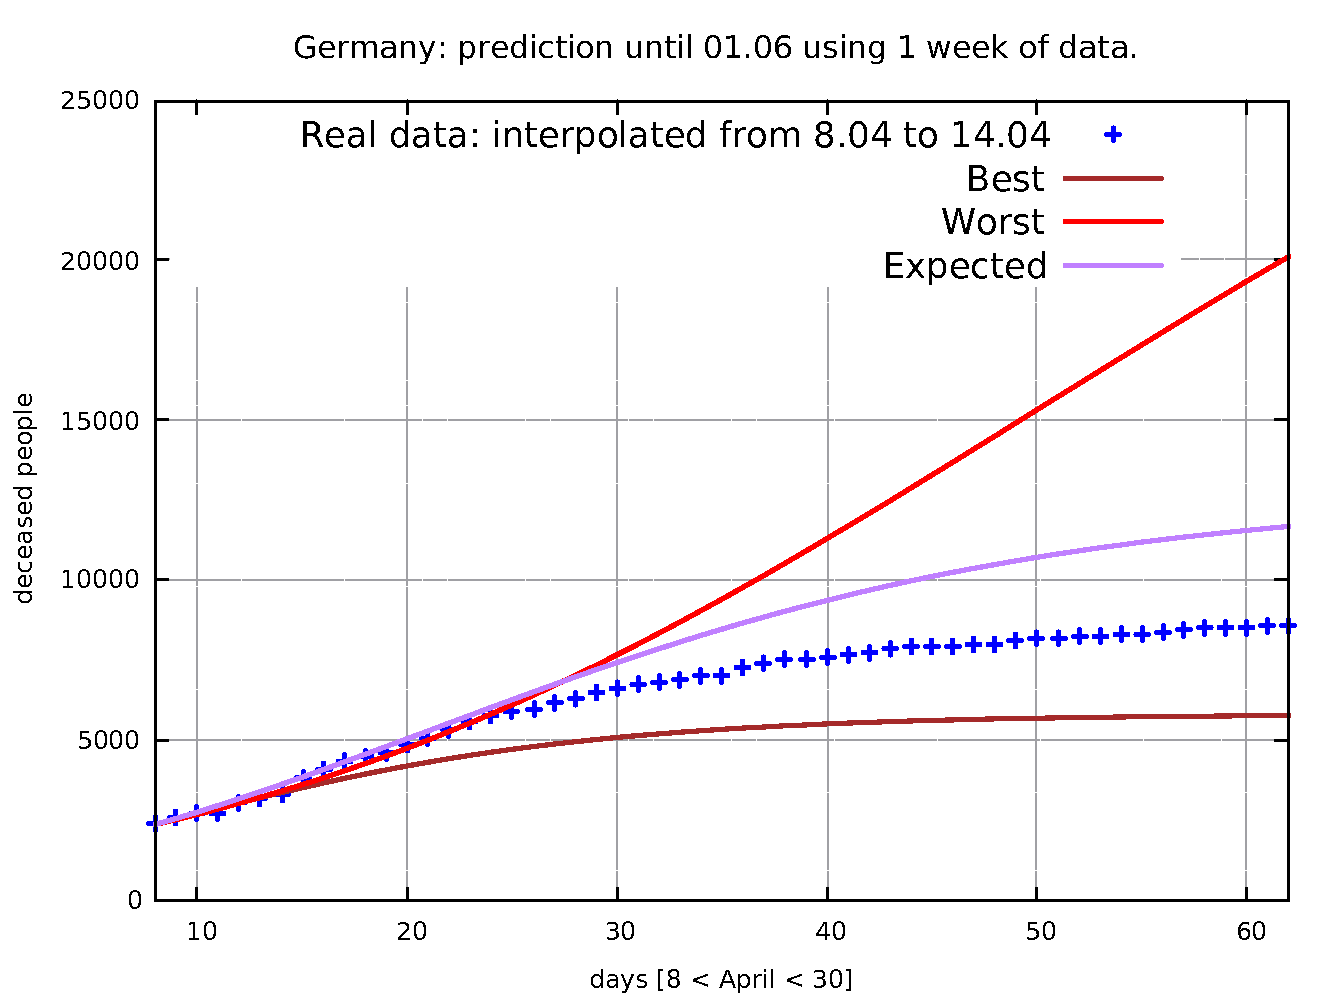
\includegraphics[width=\linewidth]{../tuned/de/8-14/8-14.pdf}
  \end{subfigure}
  \begin{subfigure}[b]{0.45\linewidth}
    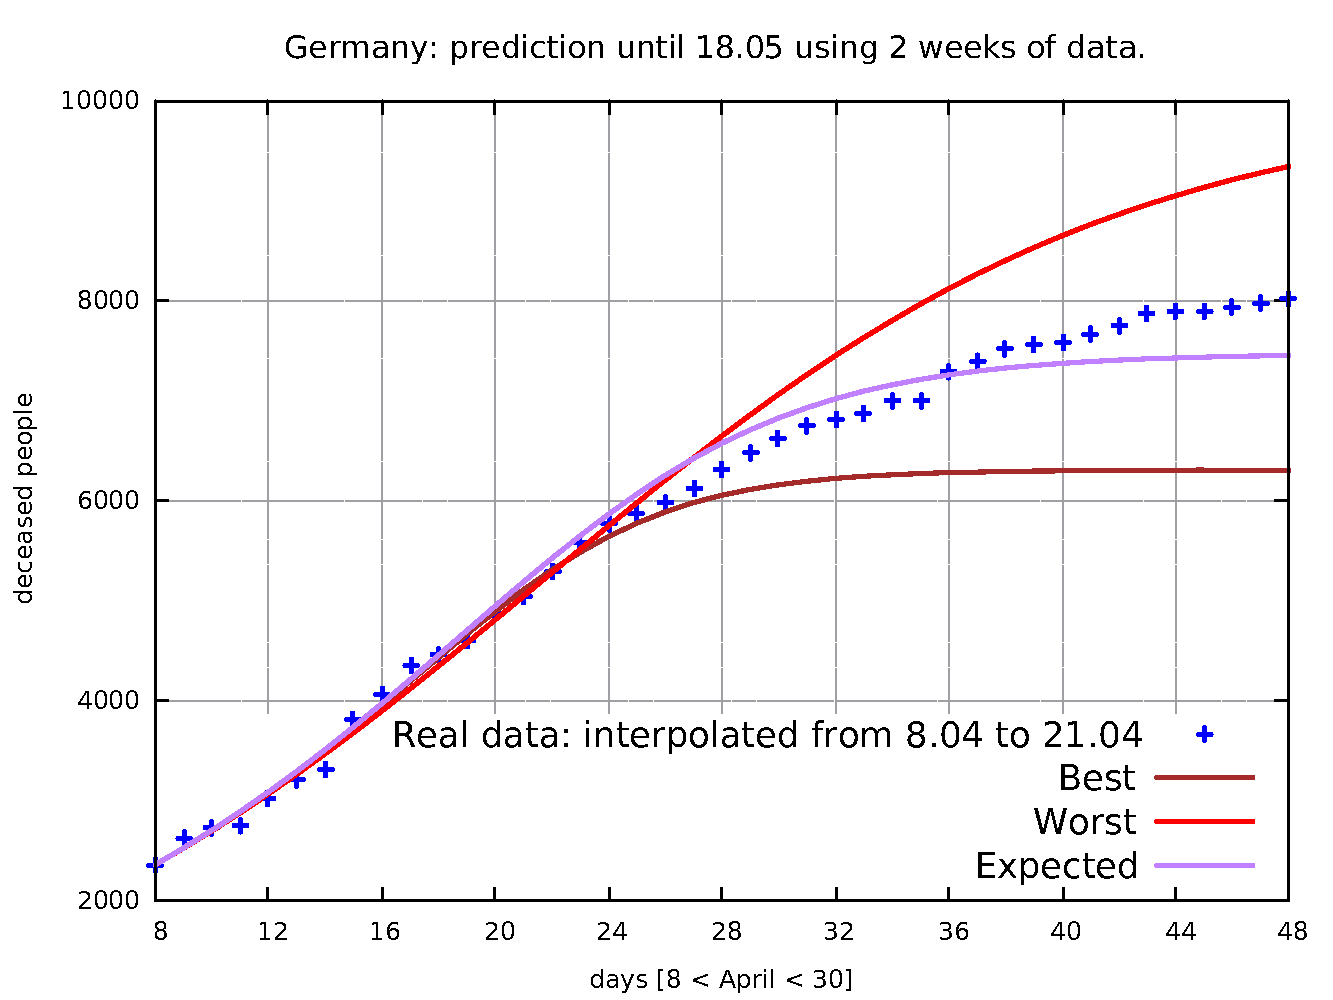
\includegraphics[width=\linewidth]{../tuned/de/8-21/8-21.pdf}
  \end{subfigure}
  \begin{subfigure}[b]{0.45\linewidth}
  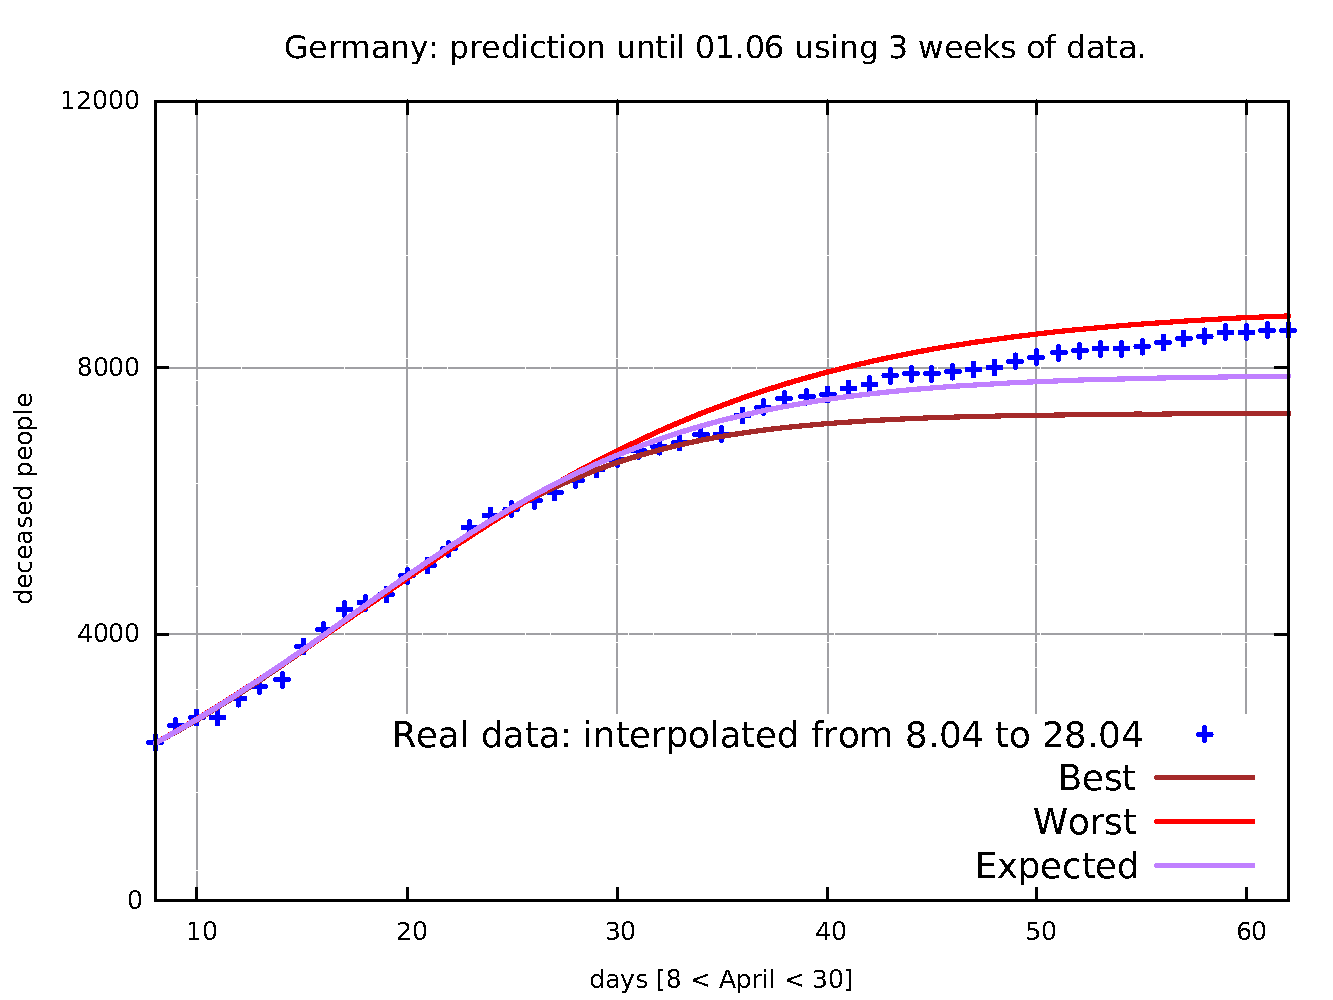
\includegraphics[width=\linewidth]{../tuned/de/8-28/8-28.pdf}
  \end{subfigure}
	\caption{Germany - to write}
\end{figure}

\begin{figure}[h!]
  \centering
  \begin{subfigure}[b]{0.45\linewidth}
  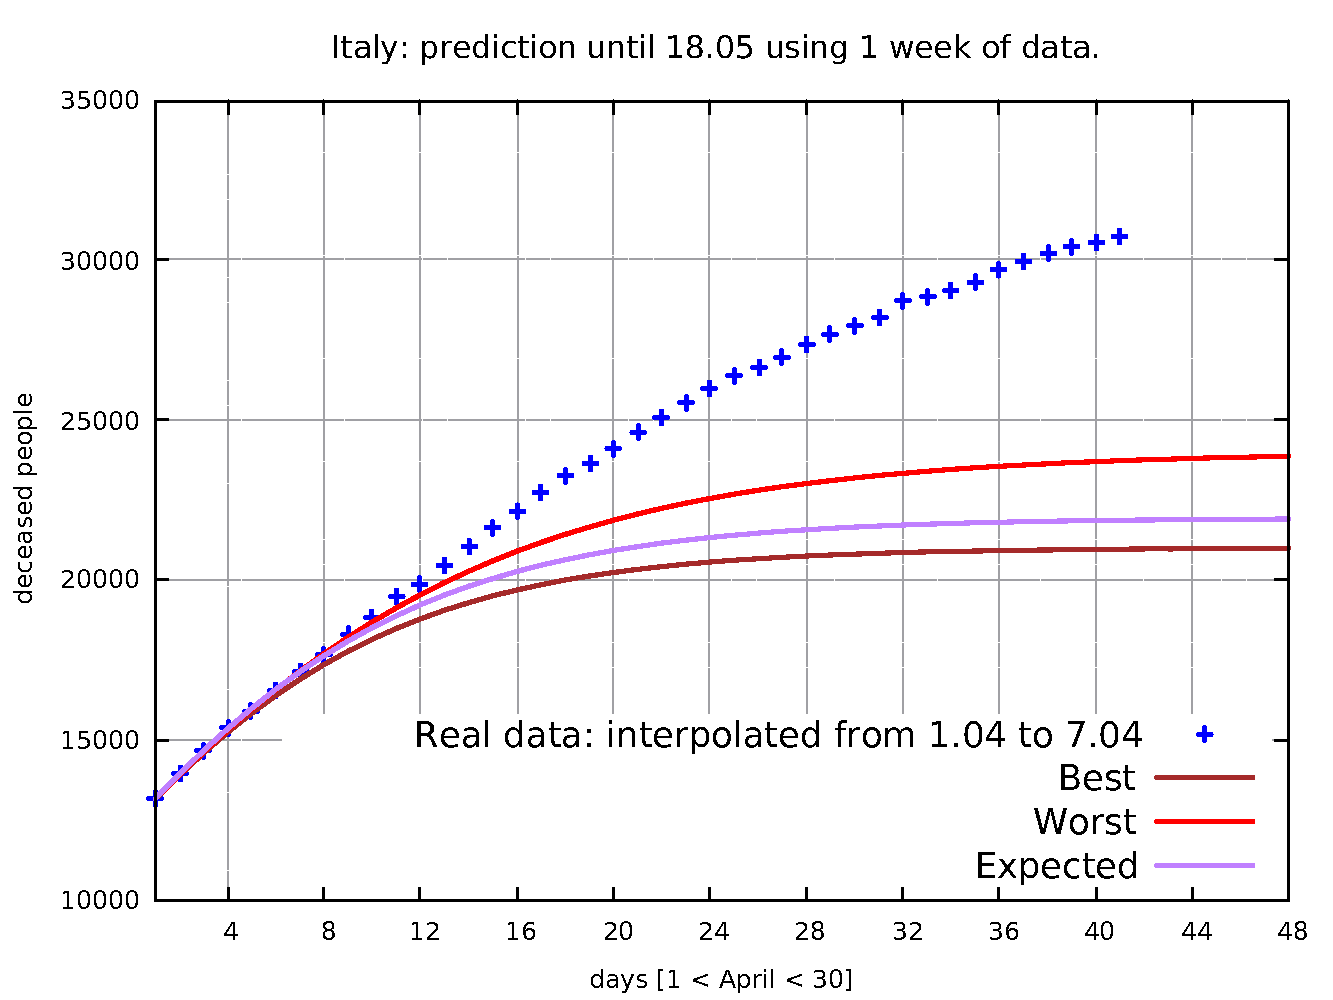
\includegraphics[width=\linewidth]{../tuned/it/1-7/1-7.pdf}
  \end{subfigure}
  \begin{subfigure}[b]{0.45\linewidth}
    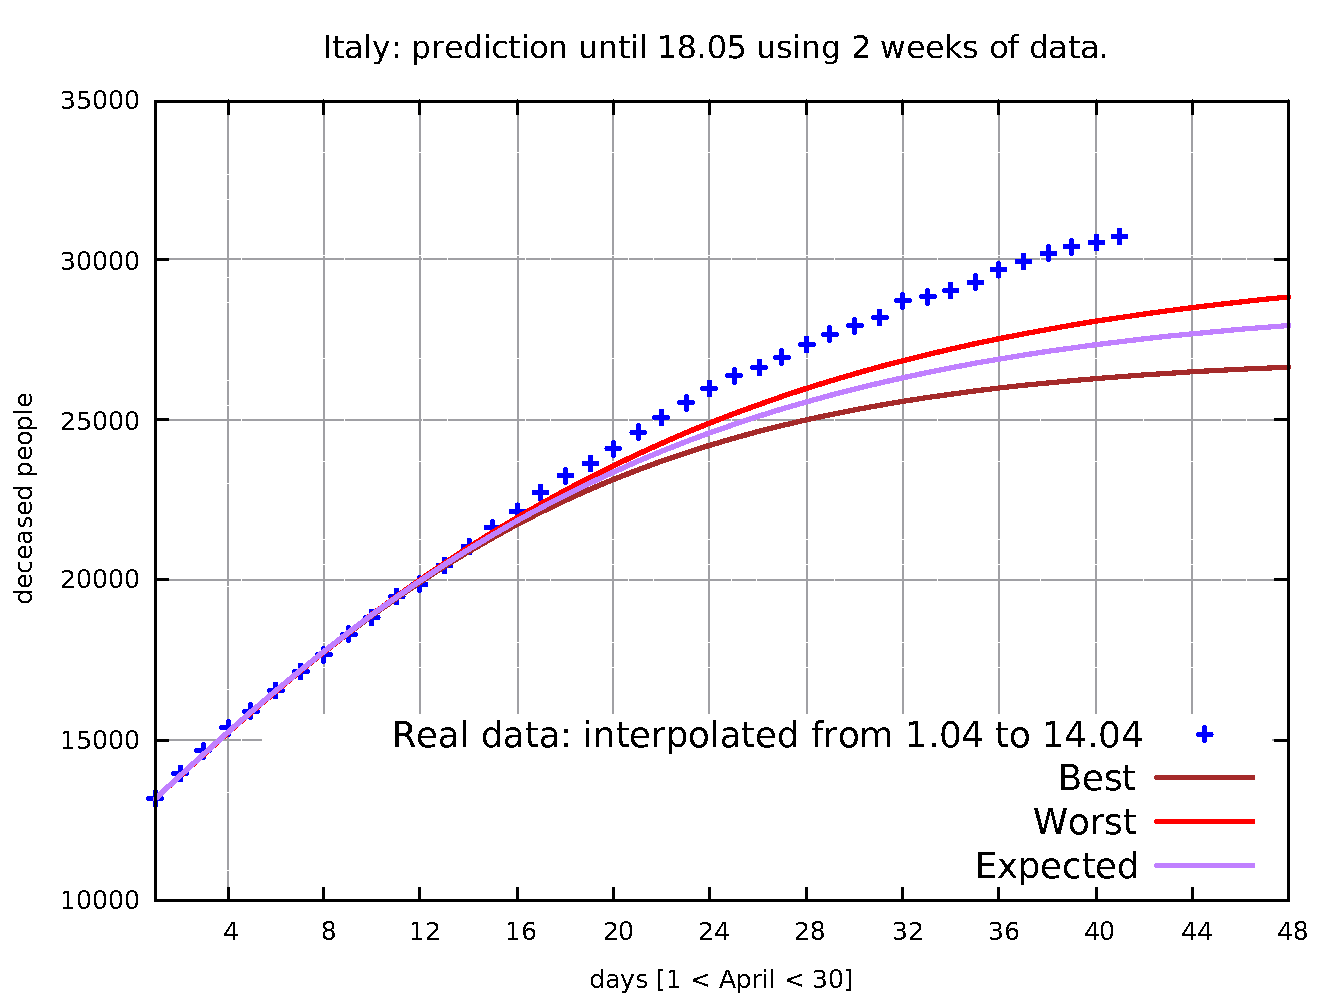
\includegraphics[width=\linewidth]{../tuned/it/1-14/1-14.pdf}
  \end{subfigure}
  \begin{subfigure}[b]{0.45\linewidth}
  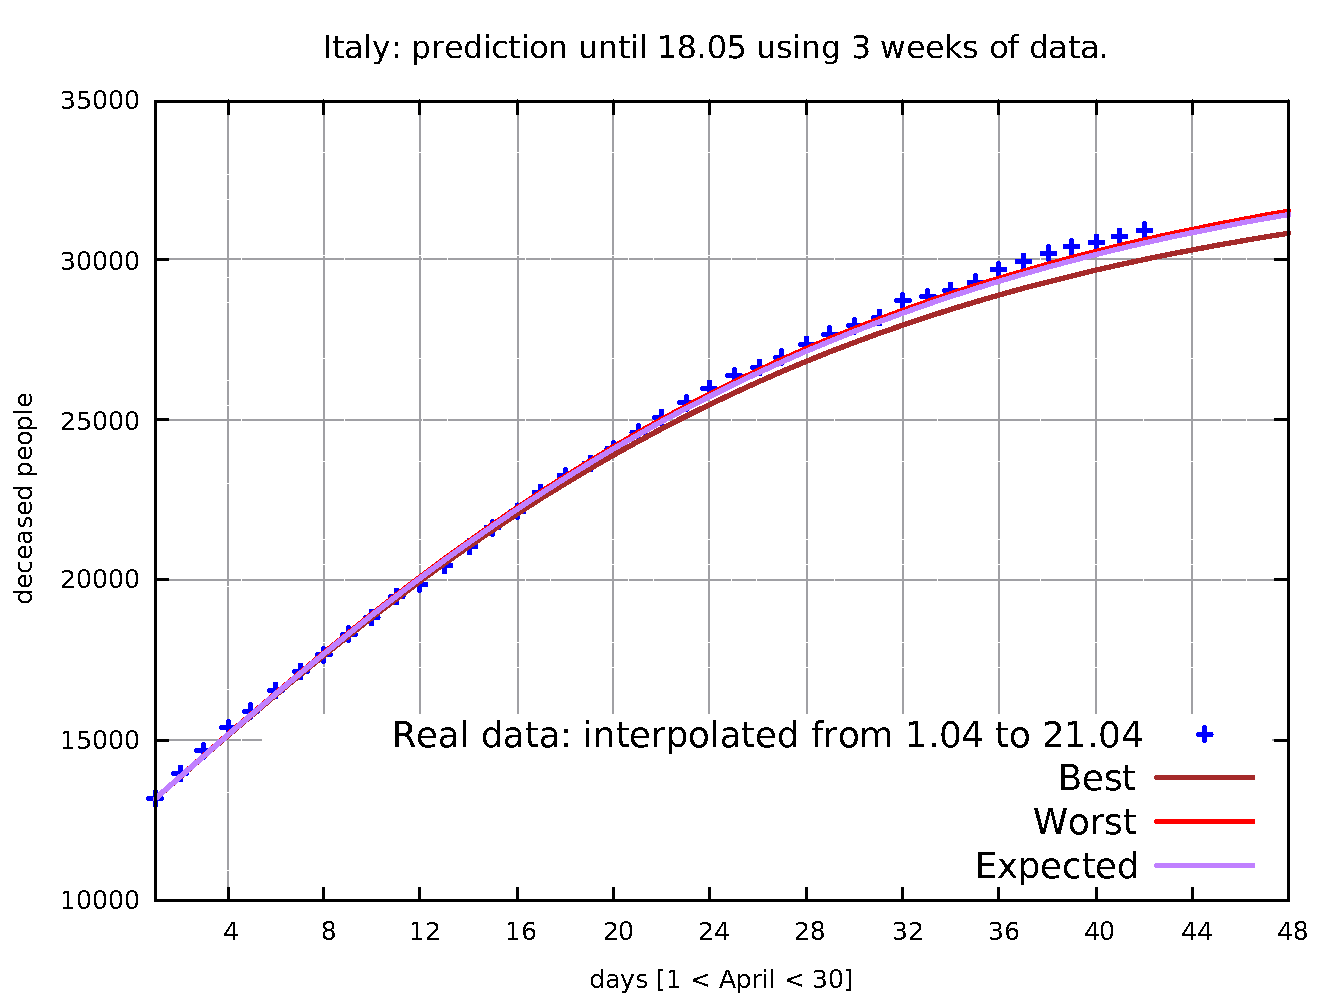
\includegraphics[width=\linewidth]{../tuned/it/1-21/1-21.pdf}
  \end{subfigure}
	\caption{Italy - to write}
\end{figure}

\begin{figure}[h!]
  \centering
  \begin{subfigure}[b]{0.45\linewidth}
  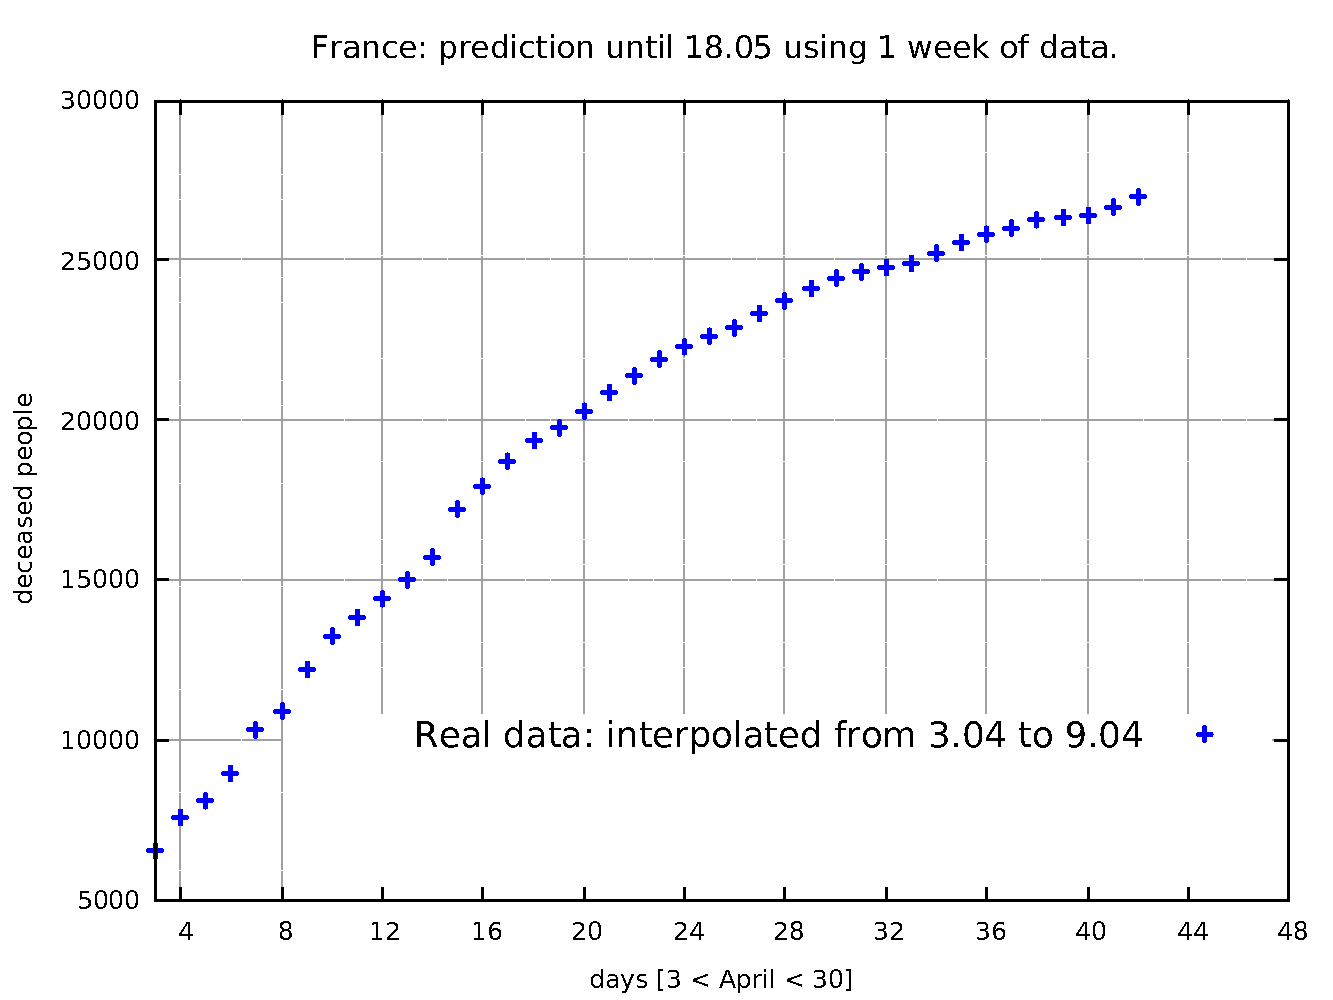
\includegraphics[width=\linewidth]{../tuned/fr/3-9/3-9.pdf}
  \end{subfigure}
  \begin{subfigure}[b]{0.45\linewidth}
    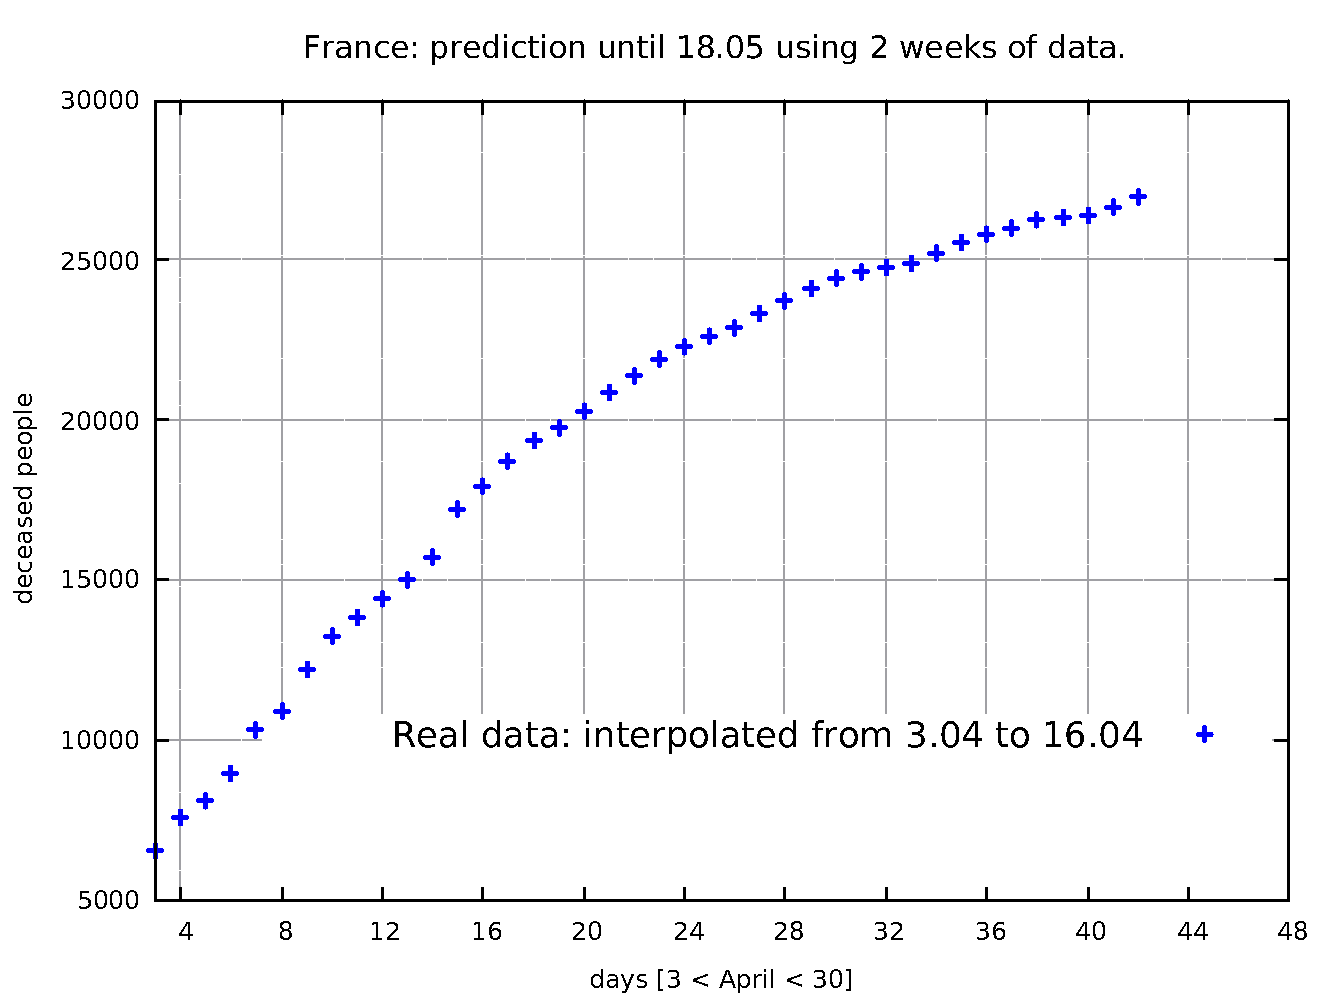
\includegraphics[width=\linewidth]{../tuned/fr/3-16/3-16.pdf}
  \end{subfigure}
  \begin{subfigure}[b]{0.45\linewidth}
  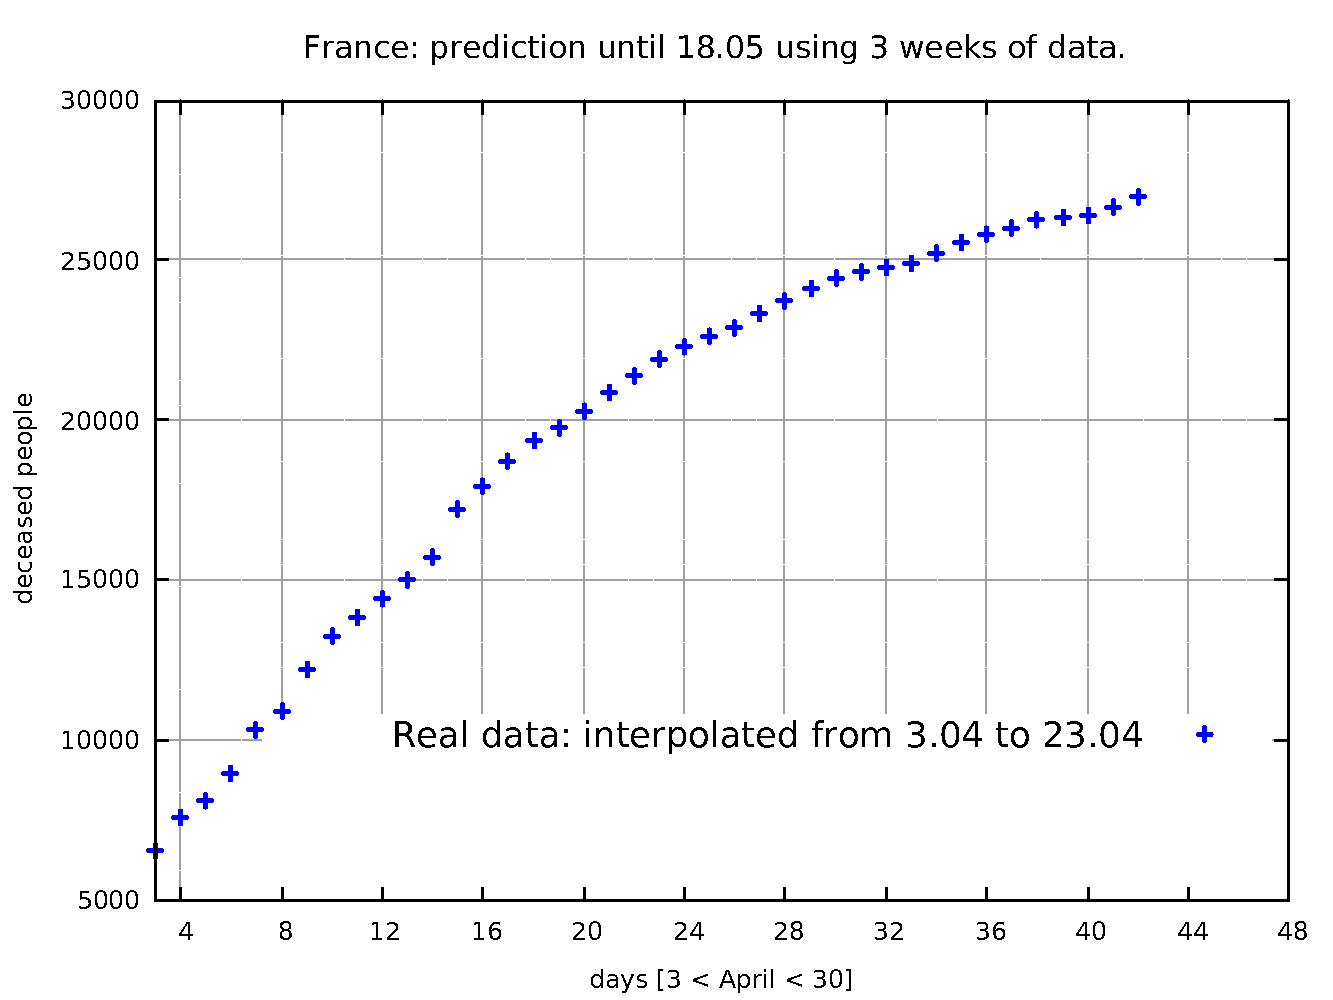
\includegraphics[width=\linewidth]{../tuned/fr/3-23/3-23.pdf}
  \end{subfigure}
	\caption{France - to write}
\end{figure}


\begin{figure}[h!]
  \centering
  \begin{subfigure}[b]{0.45\linewidth}
  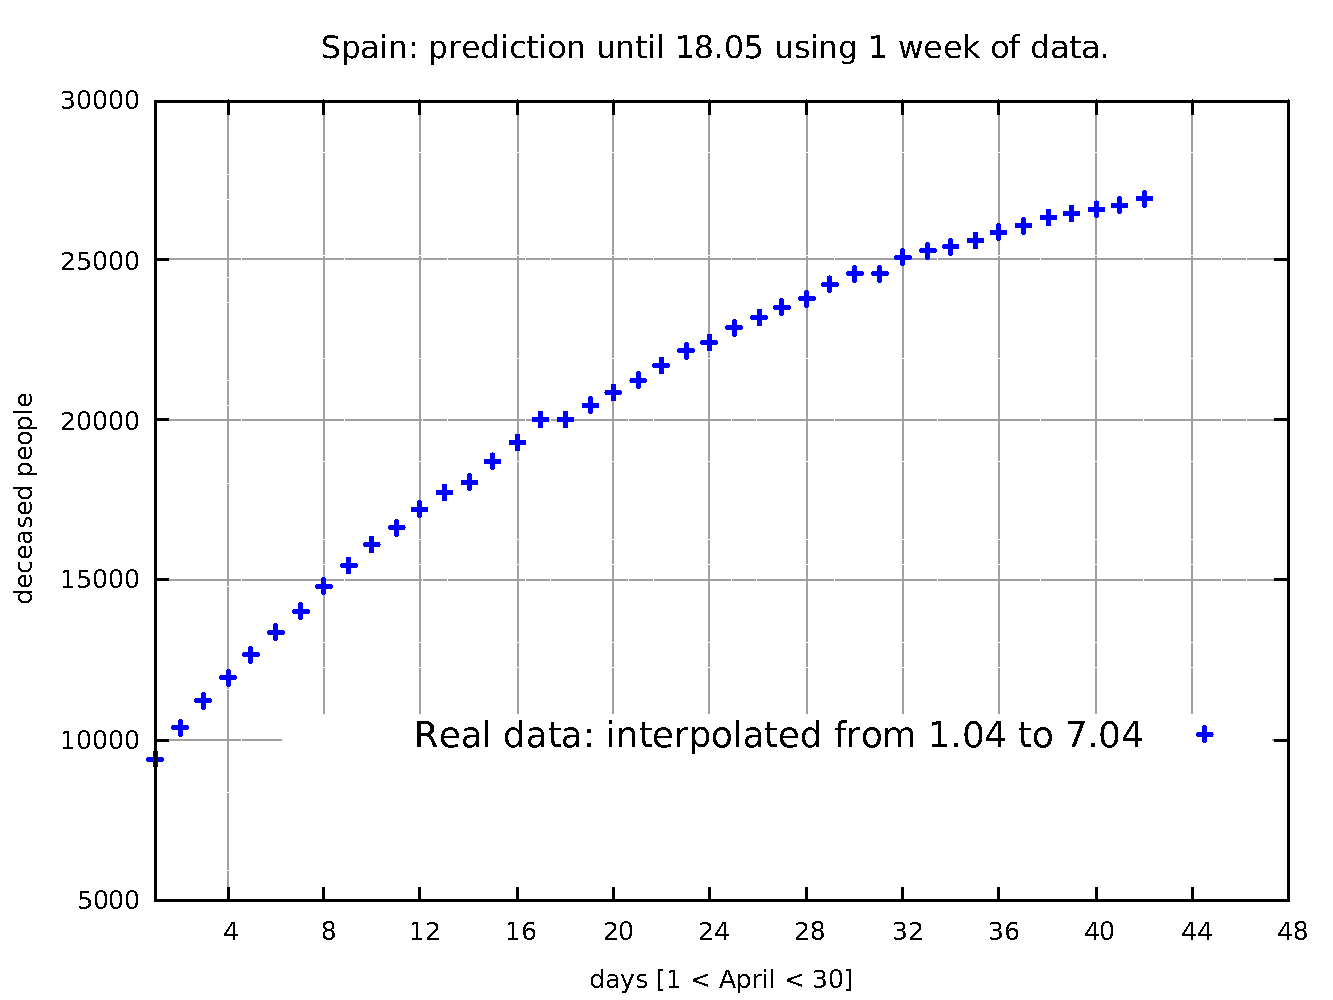
\includegraphics[width=\linewidth]{../tuned/sp/1-7/1-7.pdf}
  \end{subfigure}
  \begin{subfigure}[b]{0.45\linewidth}
    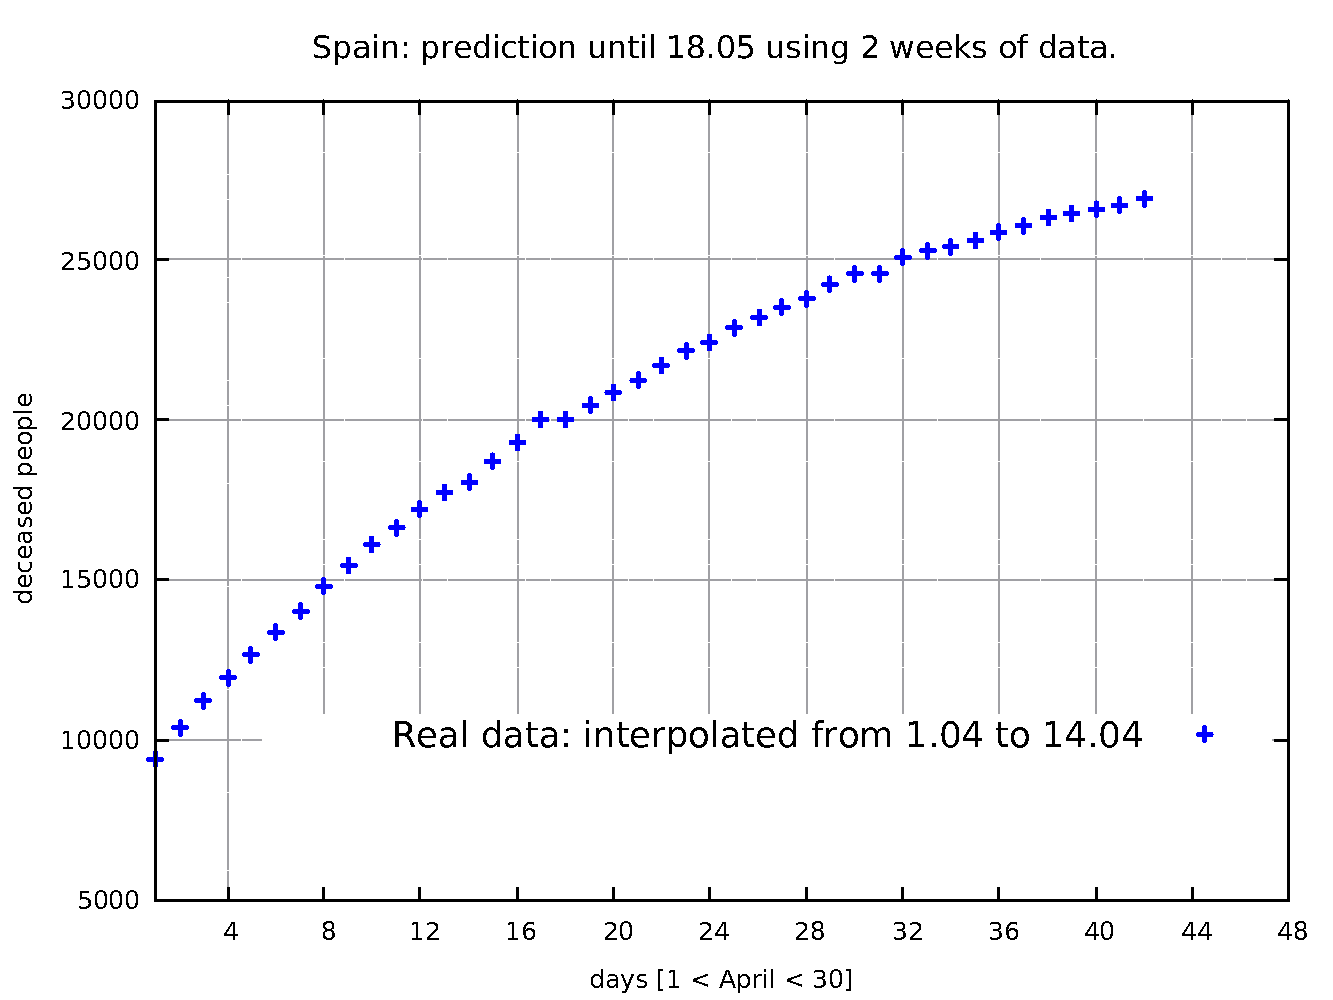
\includegraphics[width=\linewidth]{../tuned/sp/1-14/1-14.pdf}
  \end{subfigure}
  \begin{subfigure}[b]{0.45\linewidth}
  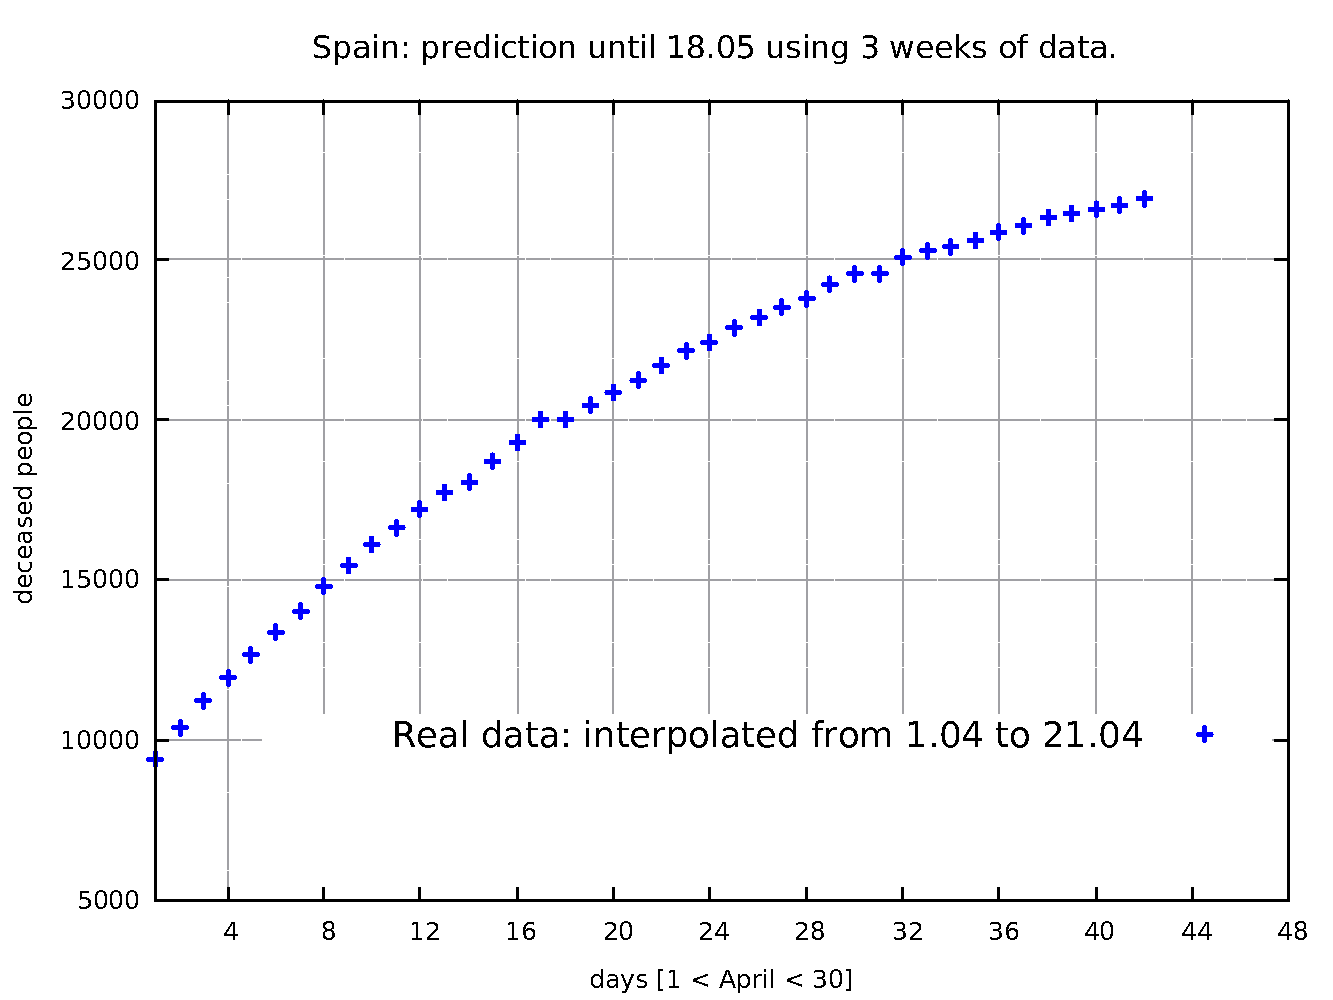
\includegraphics[width=\linewidth]{../tuned/sp/1-21/1-21.pdf}
  \end{subfigure}
	\caption{Spain - to write}
\end{figure}


\begin{figure}[h!]
  \centering
  \begin{subfigure}[b]{0.45\linewidth}
  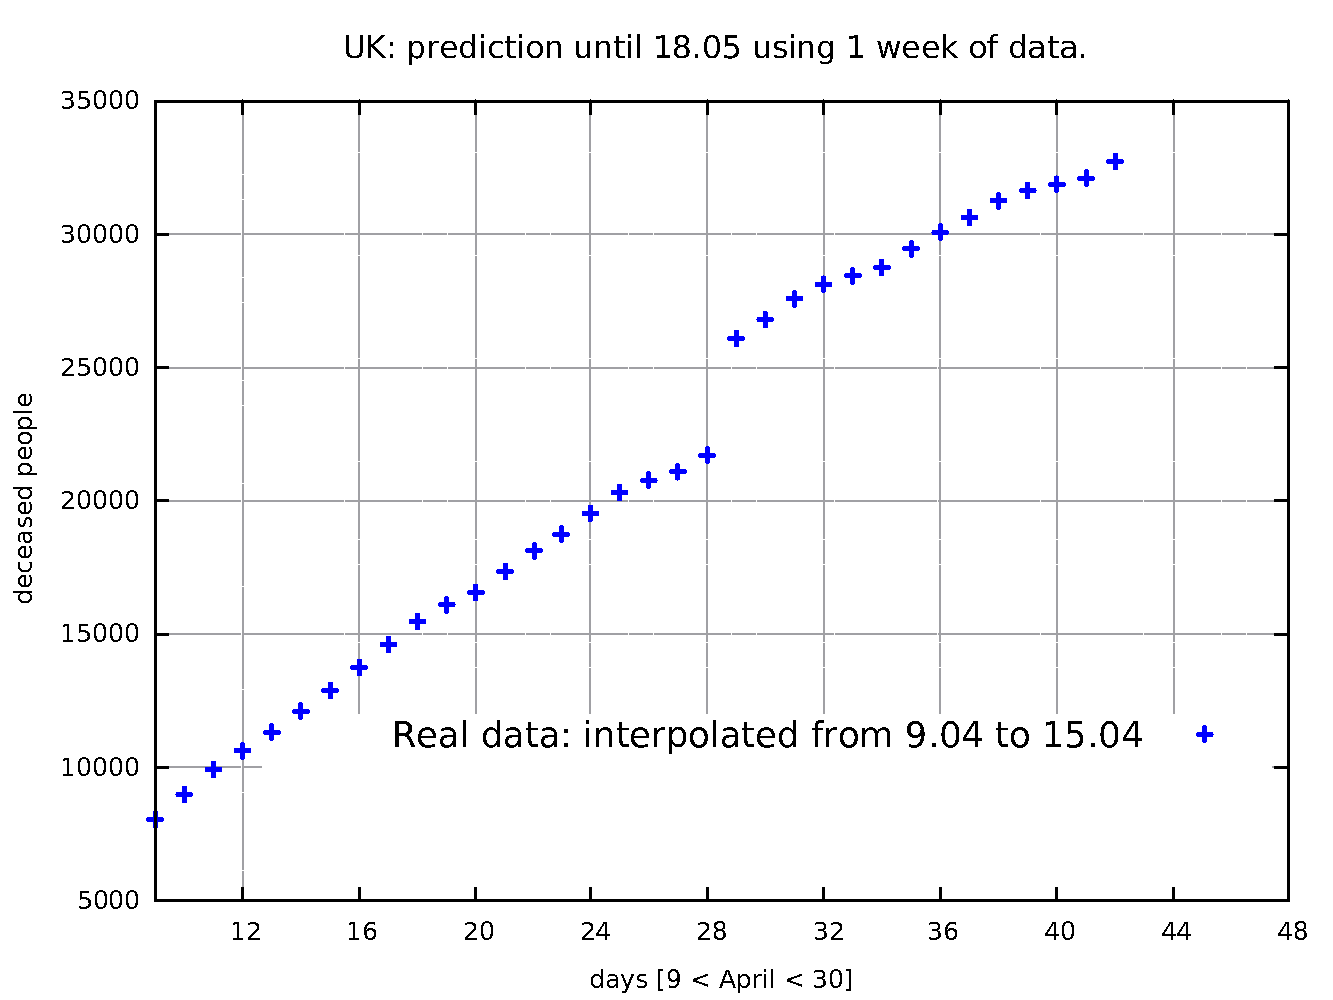
\includegraphics[width=\linewidth]{../tuned/uk/9-15/9-15.pdf}
  \end{subfigure}
  \begin{subfigure}[b]{0.45\linewidth}
    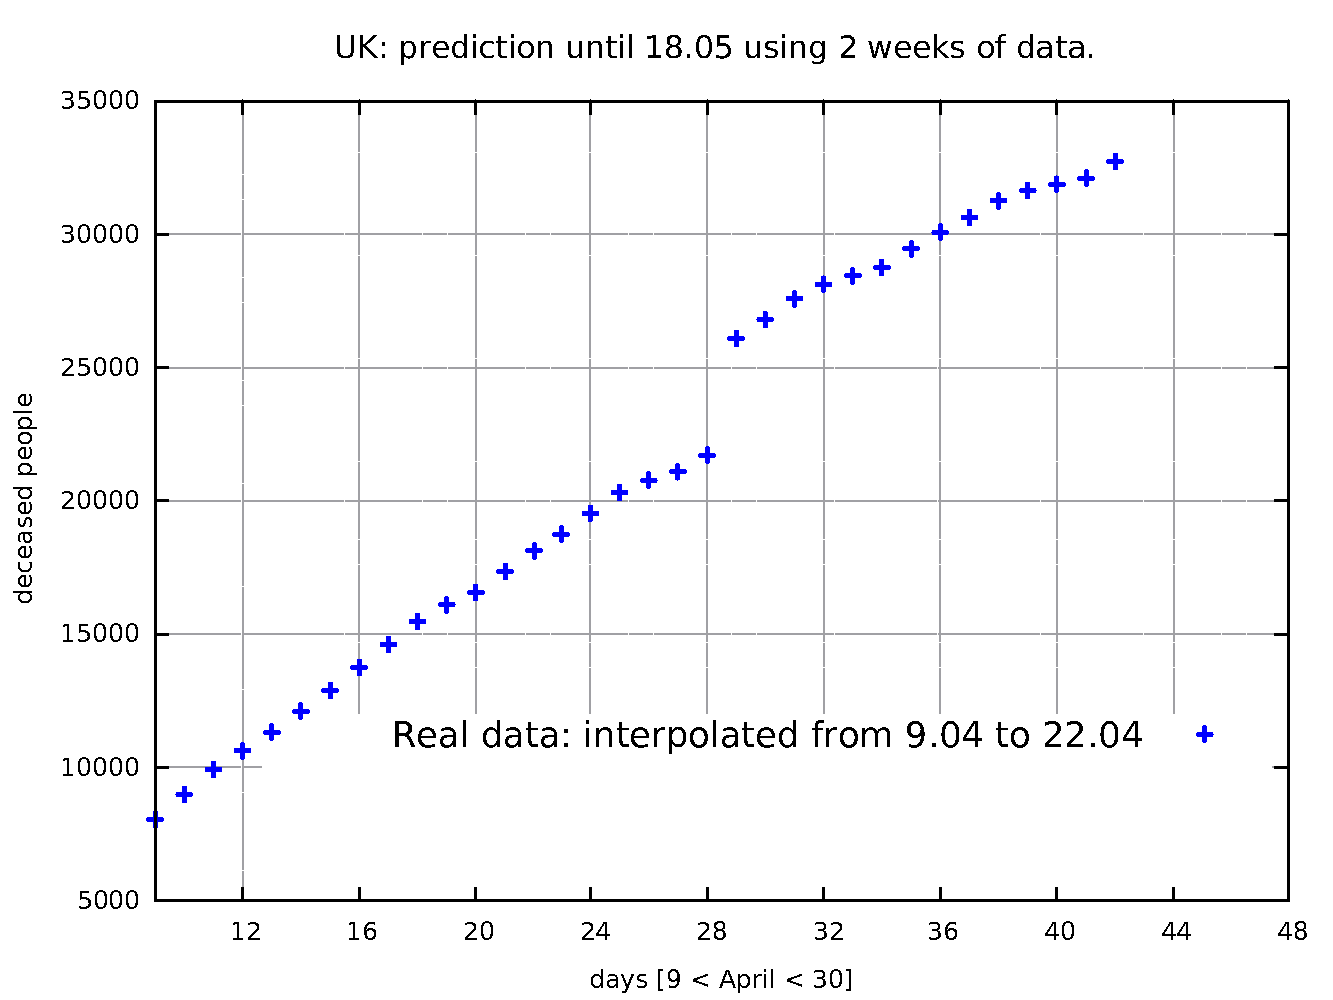
\includegraphics[width=\linewidth]{../tuned/uk/9-22/9-22.pdf}
  \end{subfigure}
  \begin{subfigure}[b]{0.45\linewidth}
  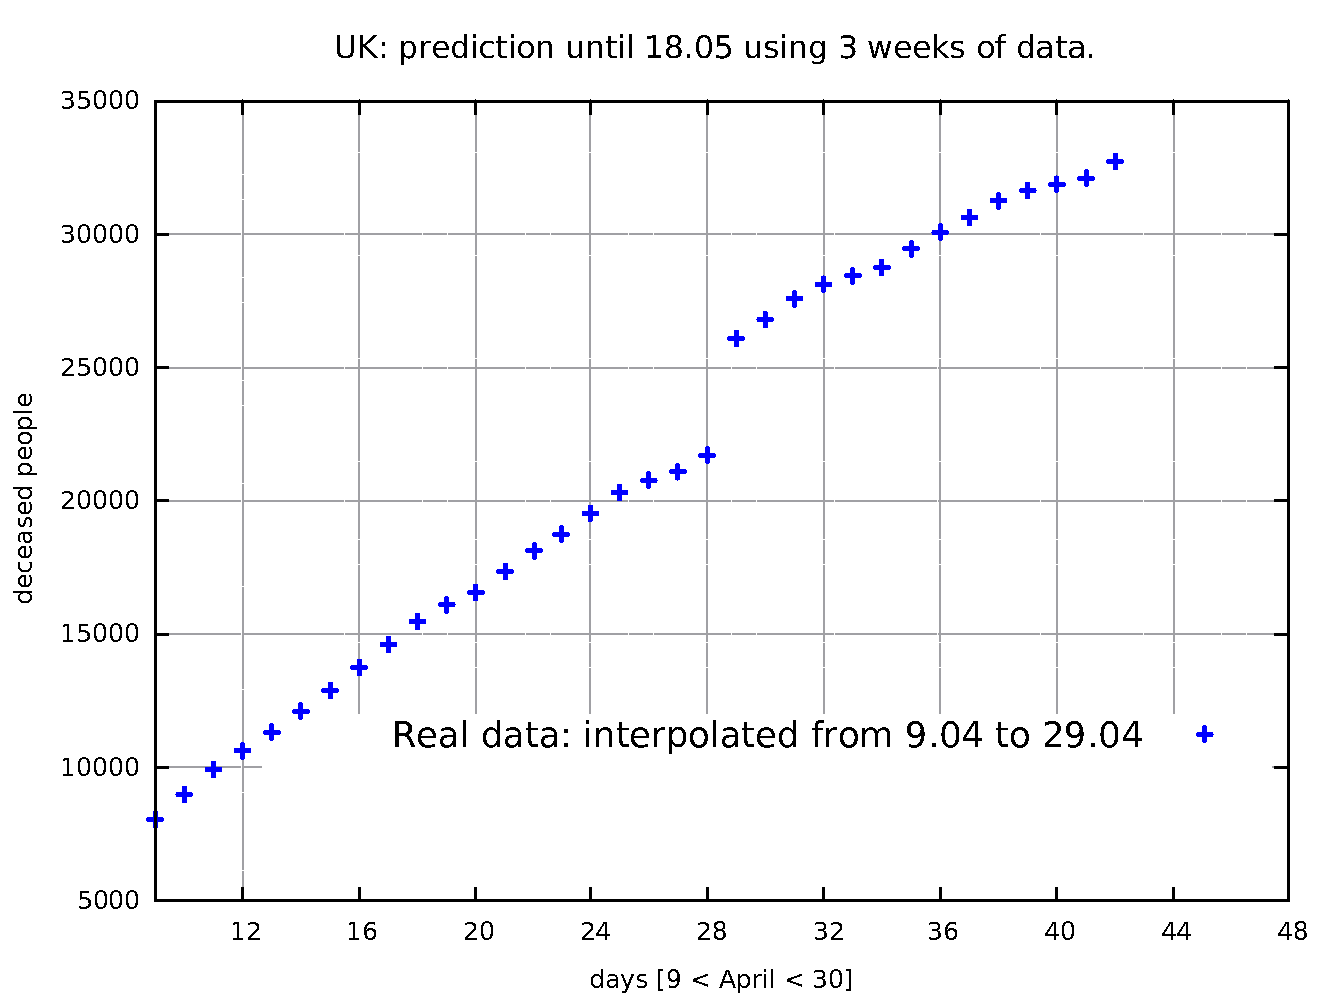
\includegraphics[width=\linewidth]{../tuned/uk/9-29/9-29.pdf}
  \end{subfigure}
	\caption{UK - to write}
\end{figure}


\end{document}
